\documentclass[12pt]{scrartcl}
\usepackage{geometry}
\geometry{margin=1in}
\usepackage{xcolor}
\usepackage{enumitem}
\setlist{nosep}
\usepackage{tikz}
\usetikzlibrary{arrows.meta, positioning}
\usepackage{iftex}
% breakurl uses pdftex-specific primitives; load it only when using pdfTeX.
% For XeLaTeX/LuaLaTeX use the standard url package (hyperref will work with it).
\ifPDFTeX
  \usepackage{breakurl}
\else
  \usepackage{xurl} % better automatic URL breaking for XeLaTeX/LuaLaTeX
  \usepackage{url}
\fi
% Allow line breaking in URLs and long links
\def\UrlBreaks{\do\/\do-\do_\do.\do:\do?\do&\do\%}
\setlength\Urlmuskip{0mu plus 1mu}
\usepackage[breaklinks=true]{hyperref}
% Allow graphics filenames with multiple dots or spaces
\usepackage{grffile}
\usepackage{graphicx}


\begin{document}
% \section*{Kohiki Slip Slab Building and Wood-Fired Soda Firing}

\section*{Lesson Plan: Kohiki Slip Decoration for Slab Building}

\subsection*{Objectives}
\begin{itemize}
  \item Introduce participants to the history and aesthetics of kohiki slip decoration.
  \item Teach slab-building fundamentals with emphasis on surface treatment.
  \item Guide students through applying kohiki slip and integrating it into functional or sculptural forms.
\end{itemize}

\subsection*{Materials}
\begin{itemize}
  \item Clay body (dark stoneware recommended).
  \item White slip (prepared to a thick cream consistency).
  \item Brushes, sponges, etc\ldots
  \item Straight edges, rulers, tar paper for patterns.
  \item Rolling pins or slab roller.
  \item Canvas boards for rolling slabs.
  \item Wooden boards for working surfaces.
  \item Bevel cutters, knives, and scoring tools.
  \item Reference images of kohiki ware.
\end{itemize}

\subsection*{Activities}
\begin{enumerate}
  \item \textbf{Introduction (20 min)}: Brief history of kohiki slip; show examples.
  \item \textbf{Slab Preparation (20 min)}: Demonstrate rolling slabs evenly; discuss thickness control.
  \item \textbf{Slip Application (60 min)}: Demonstrate brushing, dipping, or pouring slip; encourage freedom and experimentation--see discussion and exercises below.
  \item \textbf{Lunch and Patience ($\approx$1.5 hr)}: Allow time for slip and clay to firm up.
  \begin{itemize}
    \item \textbf{Structured Lunch/Throwing Demo (40 min)}: Provide short guided exercises students can do while waiting.
    \item \textbf{Structured Lunch/Practice Slot (20–30 min)}: Provide short guided exercises students can do while waiting.
    \subitem \textbf{--Goal}: Turn downtime into deliberate practice focused on slip observation and simple brushwork.
  \end{itemize}
  \item \textbf{Discussion on Leatherhard Stage (20 min)}: Talk about ideal leatherhard conditions for construction; show examples.
  \item \textbf{Slab Construction (1 hr)}: Demonstrate joining slabs into simple forms; emphasize scoring and compression.
  \item \textbf{Wrap-Up Discussion (15 min)}: Share results; discuss how kohiki surfaces change in firing.
\end{enumerate}

\subsection*{Teaching Notes}
\begin{itemize}
  \item Stress patience: kohiki slip rewards subtlety.
  \item Encourage integration of surface decoration with form.
  \item Highlight how firing atmosphere alters slip appearance.
\end{itemize}

% ---------------------------------------------------------------------------
\section*{Kohiki Slip}

\scalebox{.7}{
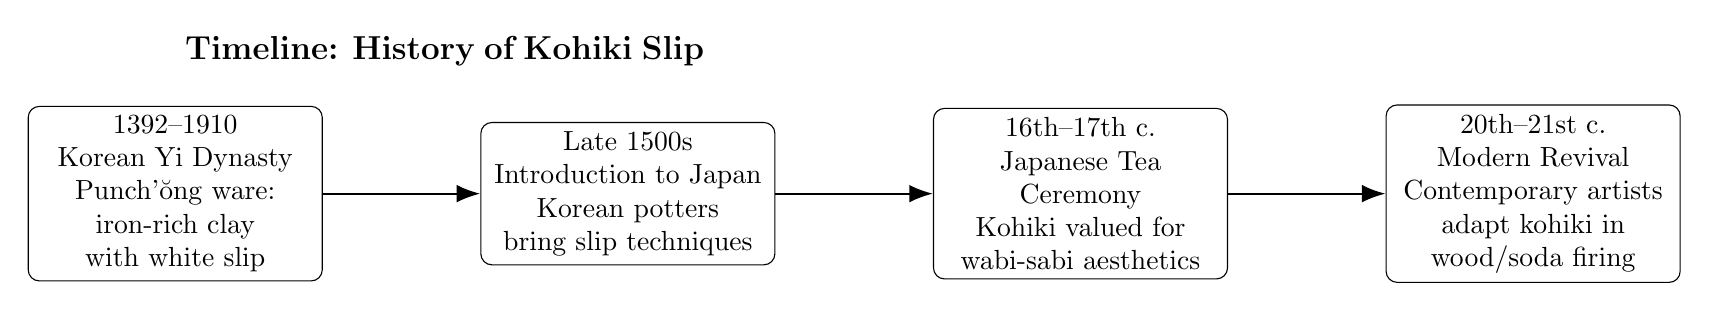
\begin{tikzpicture}[
  timeline/.style={rectangle, draw, rounded corners, align=center, text width=3.5cm},
  arrow/.style={-{Latex[length=3mm]}, thick}
]

% Nodes
\node[timeline] (yi) {1392--1910 \\ Korean Yi Dynasty \\ Punch'ŏng ware: iron-rich clay with white slip};
\node[timeline, right=2cm of yi] (japan) {Late 1500s \\ Introduction to Japan \\ Korean potters bring slip techniques};
\node[timeline, right=2cm of japan] (tea) {16th--17th c. \\ Japanese Tea Ceremony \\ Kohiki valued for wabi-sabi aesthetics};
\node[timeline, right=2cm of tea] (modern) {20th--21st c. \\ Modern Revival \\ Contemporary artists adapt kohiki in wood/soda firing};
\node[above=1cm of yi, align=left, anchor =north west, text width=9cm] {\textbf{\large Timeline: History of Kohiki Slip}};

% Arrows
\draw[arrow] (yi) -- (japan);
\draw[arrow] (japan) -- (tea);
\draw[arrow] (tea) -- (modern);

\end{tikzpicture}
}\\[5pt]


\scalebox{.7}{
\begin{tikzpicture}[
  timeline/.style={rectangle, draw, rounded corners, align=center, text width=3.5cm},
  arrow/.style={-{Latex[length=3mm]}, thick}
]

% Nodes
\node[timeline] (imjin) {1592--1598 \\ Imjin Wars \\ Toyotomi Hideyoshi invades Korea};
\node[timeline, right=2cm of imjin] (migration) {Late 1500s--early 1600s \\ Forced Migration \\ Thousands of Korean potters relocated to Japan};
\node[timeline, right=2cm of migration] (techniques) {17th c. \\ Transmission of Techniques \\ Punch’ŏng slip, porcelain, celadon introduced};
\node[timeline, right=2cm of techniques] (integration) {17th--18th c. \\ Integration into Japanese Ceramics \\ Kohiki, Arita porcelain, and hybrid styles emerge};
\node[above=1cm of imjin, align=left, anchor =north west, text width=20cm] {\textbf{\large Parallel Timeline: Import of Korean and Chinese Potters to Japan}};

% Arrows
\draw[arrow] (imjin) -- (migration);
\draw[arrow] (migration) -- (techniques);
\draw[arrow] (techniques) -- (integration);

\node[timeline, below=2cm of tea] (shino) {Late 1500s--early 1600s \\ Shino Ware Development \\ Mino region, Japan’s first white glaze pottery, parallel to Kohiki};
\draw[arrow, dashed] (japan) -- (shino);
\draw[arrow, dashed] (shino) -- (integration);

\end{tikzpicture}
}\\[7pt]

A couple modern examples of popular kohiki slip decoration by Akira Satake and Robert Fornell, as shown in the images below.  I started experimenting with kohiki slip decoration after seeing Satake's work.
\begin{center}
    \includegraphics[width=0.45\textwidth]{"0E86D316-7988-4B0F-956F-CD873AA9155E.jpg"}\qquad\includegraphics[width=0.45\textwidth]{"Screenshot 2025-11-24 205841.png"}
\end{center}

\newpage

A beautiful example of a more traditional kohiki piece is this tea bowl identified as Agano ware on this website: \url{https://qualitychanoyu.com/2023/01/13/antique-agano-ware-kobiki-chawan/}
\begin{center}
    \includegraphics[width=0.5\textwidth]{"Screenshot 2025-11-24 204241.png"}
\end{center}


Other links of interest about kohiki ware:
\begin{itemize}
  \item \url{https://turuta.jp/ceramics-story/archives/21164}
  \item \url{https://dawan-chawan-chassabal.blogspot.com/2010/02/powdery-matsudaira-at-hatakeyama-museum.html}
  \item \url{https://dawan-chawan-chassabal.blogspot.com/2010/11/powdery-matsudaira-revisited.html}\\[5pt]
\end{itemize}

Although Europeans later came to prize East Asian porcelain and reshaped its markets, the white surfaces used in Punch'ŏng and kohiki developed within East Asia before Europeans had sustained contact. These white‑slip techniques grew from local aesthetics and kiln practice, not from European influence. European demand in the 17th–19th centuries expanded export production in China and inspired European porcelain manufacture, but it did not influence Korea’s (and later Japan’s shino ware) white‑slip aesthetics.

\clearpage
\subsection*{Slab Thickness: Importance and Tradeoffs}

The thickness of your clay slab is important for both the construction process and the final appearance of your work. 

\begin{itemize}
  \item \textbf{Structural Integrity}: Thicker slabs are less prone to warping and cracking during handling and drying, making them more forgiving for experimental work or for larger forms.
  \item \textbf{Workability}: Thinner slabs are easier to bend, shape, and join, but require more careful handling to avoid tearing or distortion during firing.
  \item \textbf{Surface Techniques}: Very thin slabs may dry too quickly for certain slip or texture applications, while thick slabs can retain moisture longer, allowing more time for surface work.
  \item \textbf{Aesthetics}: The visual weight and tactile feel of the finished piece are directly affected by slab thickness. Thicker walls can feel more robust, while thinner ones may appear more delicate or refined.
\end{itemize}

\textbf{Tradeoff}: Choose slab thickness based on your intended technique and form. For kohiki slip decoration, a medium thickness (typically 6-8\,mm) balances workability, surface quality, and structural strength. Always test and adjust based on your clay body and project needs.

\textcolor{red}{Add discussion here about below material!}

\subsection*{Practice (30--40 min)}
Keep materials minimal: work on wooden bats for slip applications.
\begin{enumerate}
  \item \textbf{Single-Stroke Studies (6 min)}: Make one confident stroke across the bat--experiment with pressure and angle.
  \item \textbf{Opacity Ladder (6 min)}: Apply 3 horizontal bands with decreasing slip thickness (heavy → medium → thin). Let dry and note differences.
  \item \textbf{Quick Pair Share (3 min)}: Swap bats with a partner; each gives one suggestion for the other's next step.
  \item \textbf{Identify Area for Cutting and Construction (3 min)}: On your bat, mark an area you might cut out later for slab construction; consider how the slip application will interact with form.
\end{enumerate}

\subsection*{Brushwork Patterns (Step-by-step)}
\begin{enumerate}
  \item \textbf{Stippling (6 min)}: Load brush, dab vertically using the tip only; vary density for tonal control.
  \item \textbf{Drag-and-Stop (6 min)}: Pull brush in a steady stroke, lift quickly for crisp ends.
  \item \textbf{Combing (2 min)}: Use a fork or comb dragged through semi-wet slip for parallel texture.
  \item \textbf{Ribs (2 min)}: Drag a rib or flat tool through wet slip to create texture; vary angle and pressure for different effects.
\end{enumerate}

\section*{Lunch / Patience: Guided Exercises}

\textcolor{red}{Add discussion here about below material!}

\subsection*{\textbf{Exercise}: slab forming and stretching}
For a more exaggerated \& dramatic appearance of the brush work on your slab pieces, try the following exercise during lunch or downtime:
\begin{itemize}
  \item \textbf{Slab forming}: Get a small slab of clay (about 8\,mm thick) from the instructor with kohiki slip already applied.
  \item \textbf{Stretching}: Carefully pick the small slab up from one edge and practice stretching it by carefully throwing it back down onto the table or canvas at roughly a 45 degree angle. The goal is to elongate the slab and distort the brushwork in an interesting way without tearing the clay.
  \item \textbf{Repeat}: Try this several times, varying the side you pick up from and the angle of impact. Observe how the brushwork changes with each stretch.
  \item \textbf{Notes}: Take a moment to write down your impressions about how to throw the clay to get different effects, and any challenges you faced in keeping the slab intact and well textured.
\end{itemize}



\subsection*{Slip Consistency \& Quick Recipe}
\begin{itemize}
\item Basic Kohiki Slip Recipe:\\[2pt]
    \begin{tabular}{@{}ll@{}}
        EPK kaolin:      & 500 g \\
        OM4 ball clay:   & 400 g \\
        G-200 feldspar:  & 600 g \\
        Silica:          & 500 g \\
    \end{tabular}
  \item Water: variable--depends on deflocculant use if any.
  \begin{enumerate}
    \item Thin toothpaste consistency
    \item Thick cream consistency
    \item Any range in between depending on your application style and decorative goals
  \end{enumerate}
  \item Deflocculant (sodium silicate or Darvan): 1--3 g, if needed to thin without settling\footnote{Deflocculants help reduce the amount of water needed, but can reduce the workability of the clay beneath the slip. Use sparingly and test.}
\end{itemize}

\textcolor{red}{Add discussion here about below material!}

\subsection*{Quick Tests}
\begin{itemize}
  \item \textbf{Brush-Load Test}: Dip brush and make a 10 cm stroke; note opacity and pooling.
  \item \textbf{Adhesion Test}: Apply slip to a scrap of the class body, bend gently when leatherhard—does it crack or flake?
  \item \textbf{Drying Rate}: Make a thin swatch and time until it is no longer tacky—record for next session.
  \item \textbf{Hypothesis}: Suggest one hypothesis on slip application and test.
\end{itemize}

\subsection*{Observation Prompts}
\begin{itemize}
  \item Changes in color/value as the slip dries.
  \item Areas of pooling vs even coverage.
  \item Edges where slip has feathered or pulled away.
  \item Any textural interaction where slip meets tool marks.
\end{itemize}

\textcolor{red}{Add discussion here about below material!}

\subsection*{Two Micro-lectures (5--7 min each)}
	extbf{Micro-lecture A — Aesthetics of Kohiki (5 min)}: Discuss wabi-sabi, the value of subtlety, and how controlled imperfection enhances form. Show 2--3 images and ask students to name one element they find compelling.

	extbf{Micro-lecture B — Kiln Transformations (5 min)}: Explain how wood/soda firing can change slip surface—ash deposition, reduction/oxidation effects, and how slip texture traps or resists glaze.

\subsection*{Safety \& Handling Notes}
\begin{itemize}
  \item Always wash hands after handling slips containing deflocculants.
  \item Keep sanding and dry-scraping to a minimum; use wet cleaning to avoid airborne silica.
  \item Label slip containers; avoid cross-contamination between white and colored slips.
  \item For soda firing: follow kiln-specific SDS guidance for soda ash and wear PPE when handling solutions.
\end{itemize}

\subsubsection*{What I Notice / What I Would Change (Worksheet)}
\begin{enumerate}
  \item Sample ID: \hrulefill\\
  \item Observations (3 lines): \hrulefill\\ \hrulefill\\ \hrulefill
  \item One change I would make next time: \hrulefill\\
  \item Confidence (1–5): \hrulefill
\end{enumerate}


\newpage
\section*{Lesson Plan: Wood-Fired Soda Firing}

\subsection*{Objectives}
\begin{itemize}
    \item Review fundamental principles of firing across all types of kilns.
    \item Discuss the unique characteristics of wood firing.
    \item Explain the chemistry and effects of soda firing.
    \item Introduce participants to the principles of soda firing in a wood kiln.
    \item Teach preparation of work for soda atmosphere (wadding, glazing, placement).
    \item Explore how soda interacts with clay and slip surfaces.
\end{itemize}

\subsection*{Materials}
\begin{itemize}
  \item Bisque-fired student work (preferably with  surfaces prepped for wood+soda).
  \item Wadding materials (alumina hydrate + kaolin).
  \item Kiln shelves, posts, protective gear.
  \item Wood for firing (species discussion: pine, oak, etc.).
  \item Soda mix (soda ash + baking soda + whiting, in water) -- following the suggestions of Gail Nichols.
\end{itemize}

\subsection*{Activities}
\begin{enumerate}
  \item \textbf{Introduction (20 min)}: Explain soda firing chemistry; show examples.
  \item \textbf{Preparation of Work (30 min)}: Demonstrate wadding placement; discuss glaze choices.
  \item \textbf{Kiln Loading (45 min)}: Explain loading strategies; emphasize safety and teamwork.
  \item \textbf{Firing Process (30 min overview)}: Walk through firing stages; demonstrate soda introduction; discuss temperature targets.
  \item \textbf{Cooling \& Unloading (Next Session)}: Explain cooling protocols; plan for unloading and critique.
  \item \textbf{Wrap-Up Discussion (15 min)}: Anticipate results; encourage embracing variation and unpredictability.
\end{enumerate}

\subsection*{Teaching Notes}
\begin{itemize}
  \item Stress safety: protective gear, teamwork, kiln etiquette.
  \item Highlight unpredictability as part of the aesthetic.
  \item Connect back to constructed works: how soda atmosphere transforms surfaces.
\end{itemize}

\section*{Suggested Flow}
\begin{itemize}
  \item Works construction.
  \item Bisque firing.
  \item Soda firing preparation: kiln prep, loading, firing overview.
  \item Kiln unloading, critique, reflection.
\end{itemize}





\end{document}